\appendix
\chapter*{Appendix}
 Appendix A, B, C and D, include the interviews reports and will be provided in Norwegian only.

\section*{Appendix A - Intervju 22/10/12 kl. 1300}
\label{A}

\emph{Intervjuobjekt:}\\
Navn: Jorunn Helbostad \\
Utdannelse: Hovedfag og doktorgrad i fysioterapi, ved Universitetet i Bergen.\\
Arbeidssted: Forske på St. Olavs Hospital, Trondheim\\ \\
\emph{-Av deres pasienter fra 65 år og oppover, hva er problemet? Har dere pasienter som er hos dere for opptrening etter for eksempel en skade (rehabilitering)? Har dere pasienter som er hos dere for generell trening fordi de ønsker å styrke kroppen?}\\
Det finnes private og kommunale fysikalske klinikker. Disse har avtale med trygdesystemet. For å få time hos fysioterapeut må man ha rekvisisjon. Pasienten kommer  i kontakt med fysioterapeuter gjerne fordi de har et definert problem. Det hender for eksempel hjemmesykepleiere tar kontakt på vegne av en pasient de pleier. Det er sjeldent den eldre tar kontakt selv. \\ \\
\emph{-Hvordan er oppfølgingen under behandlingen? Hvordan er oppfølgingen etter behandlingen? Pleier dere å gi pasienten program som de må trene på hjemme mellom hver time?}\\ 
Ofte er det ikke nok å være hos fysioterapeuten 1-2 ganger i uka. Det er en utfordring å få de til å gjøre noe hjemme. De eldre ønsker gjerne å "bli friske", de er ikke veldig motiverte til å trene hjemme på egenhånd. Vanlig å oppfordre til å bevege seg mer hjemme, enten ved å gi en form for treningsprogram eller si noe som "husk å være fysisk aktiv". Dette kan være at fysioterapeuten skriver en lapp med strekmennesker som forklarer øvelser, eller et dataprogram hvor man kan sette sammen et program med øvelser og printe ut til pasienten, eller noen sier bare noe så generelt som at de må ut å bevege seg.\\ \\ 
\emph{-Opplever dere at det er pasienter som har problemer med å komme seg til behandling? Hender det dere må dra på hjemmebesøk?}\\ 
Nei, de som er dårlige til beins, får dekket drosjetransport til behandlingen. Men det er klart at mange vegrer seg for å gå ut. Det er også mange som vegrer seg for å bevege seg innendørs.\\ \\
\emph{-Er det noen som uttrykker at de ønsker hyppigere trening?}\\ 
Sjedent. De vil vel gjerne få en slags "pille/medisin" og bare bli frisk og rask.\\ \\
\emph{-Er det mange som uttrykker ensomhet/ulykkelighet?}\\ 
Det er veldig få som identifiserer seg selv som en person som er redd for å falle. I prosjekter hvor det har blitt foreslått forskjellige tiltak blir man ofte møtt med svar som "Det høres ut som en fin ting. Gi det til noen som trenger det". Det er mange som ikke sier ifra at de har falt. Å forebygge noe som "ikke har skjedd" er vanskelig. Dersom man jobber med fallforebygging, bør man ikke nevne ordet "fall". Det bør fokuseres mer på positive ting, som å styrke kropp for å kunne leke med barnebarna, gå på kafe osv.\\ \\
Det er opprettet noen treningsgrupper i Trondheim som er ment å forebygge fall. Men de reklamerer ikke med dette. I stedet reklamerer de med feks: "Vil du greie mer enn før...?".\\ \\
\emph{-Hvordan får dere høre om nye behandlingsmetoder, hjelpemidler, vektøy osv?}\\ 
Vi har "Fysioterapauten" som er et tidsskrift for fysioterapauter. Her blir stilen holdt ganske ren. Ellers er det jo også artikler i blant annet aviser og magasiner. Man drar på kurs og konferanser, men da gjerne innenfor et bestemt fagområde. Et bra sted å lansere nye produkter er kanskje på konferansene eller i "Fysioterapauten". Det er ofte snakk om etterutdanningskurs, ikke så mye om nye produkter. \\ \\
\emph{-Hva er interessen for nye ting?} \\ 
Her er det snakk om en ganske konservativ gruppe. Man vil veldig gjerne ha en dokumentasjon på at det fungerer. Produktet bør ha en lav brukerterskel. Hvor lett er det å bruke? Det må lette arbeidsmengden eller forbedre arbeidet for at det skal være interessant å ta i bruk. Man må også finne ut hvem som skal betale dette. Helsesektoren? Kommunen? Man må gjerne "stå for produktet" og klare å få fram at det er verdt å betale for. Pris på produktet har nok mye å si! \\ \\
\emph{-Må nye produkter være godkjent for medisinsk bruk?}\\ 
Et spill som dette havner litt i en gråsone. Det finnes lover og regler, men jeg tror ikke man trenger medisinsk godkjenning for å ta i bruk dette spillet.\\ \\
\emph{-Hvordan foregår en kjøpsprosess hos dere?} \\ 
Det vanligste er nok at man kjøper for å eie selv. Det er interessant å leie eller prøve produktet en viss tid for å være sikker på at det er et godt kjøp. Ofte skjer det at man kjøper inn et produkt, men så blir det gjerne liggende fordi man ikke tar seg tid til å lære det. Her kreves det opplæring! Det som også gjerne skjer er at en ivrig person tar initiativ til å kjøpe et nytt produkt og lærer seg hvordan det skal brukes, for så å kanskje slutte. De gjenværende har ikke lært seg å bruke produktet, og så blir det liggende. \\ \\
\emph{-Hender det at dere kjøper inn produkter for så å selge dem videre til kundene deres?}\\ 
Fysioterapautene kunne jo kjøpt spillet og eventuelt en lisens med på kjøpet, men jeg tror kanskje at eldre vil vegre seg for å kjøpe. Hvis kommunen så på det her som noe bra, så kunne kommunen ha kjøpt inn og lånt ut til eldre. \\ \\ Det er alltid en utfordringen med ny teknologi - hvem skal betale? Prosjekter har strandet fordi man ikke blir enige om hvem som skal betale.\\ \\ På fylkeskommunalt nivå har man hjelpemiddelsentralen. Hjelpemidler som kan lette hverdagen til folk kan bli kjøpt inn av hjelpemiddelsentralen og leid ut videre. Jeg er ikke helt sikker på hva som er grensen mellom trening og "fungere bedre i hverdagen" \\ \\
\emph{-Hva slags forhold har dere til leverandørene deres?} \\ 
På avansert utstyr kan man kjøpe serviceavtale. Men det er gjerne ingen som kjøper fordi det er for dyrt. Det er behov for oppgraderinger og oppfølging. Man ønsker gjerne tilpassede programmer, det vil gi større lyst til å prøve/bruke produktet. Sånn sett foretrekker jeg å samarbeide med små bedrifter, for da kan det være lettere.\\ \\ 
\emph{-Hva tenker dere om å bruke det videospillet som vi har beskrevet som en alternativ og annerledes behandlingsmetode \\
-for generell trening?\\
-tilpasset rehabilitering?}\\ 
For å kunne si noe om dette, ville jeg sett og prøvd spillet. For at det skulle vært interessant måtte det kunne lette arbeidsdagen min som fysioterapeut og gi meg muligheten til å tilby bedre hjelp til pasientene. Dersom jeg ikke syns øvelsene er relevante, ville jeg ikke brukt spillet. Spillet må være bedre enn det jeg kan tilby selv og øvelsene må kunne tilpasses. Når jeg har en pasient vil jeg finne ut hva som er pasientens problem ved å undersøke pasienten. Ut i fra problemet jeg finner, vil jeg legge opp et program ut ifra hver enkelt pasient. Innhold og vanskelighetsgrad må være tilpasset behovet. \\ \\ 
\emph{-Hva slags verdi tror du er bevegelsesstyrkende videospill kunne gitt til en bruker?}\\ 
Det kan oppleves både som spennende og som en barriere for pasienten. Mange eldre opplever teknologi som en barriere. Spillet må fenge pasienten. Spillet bør ha mulighet for individuell tilpasning. For å redusere fall bør øvelsen inneholde balanse og styrke og det må være mulig å tilpasse vanskelighetsgrad slik at det kan bli vanskeligere. Med øvelser med fokus på styrke og balanse er det bevist at man kan redusere fall med 20-60 prosent. Det teknologi kan bidra til er å gjøre det mer underholdende og motiverende. Tilbakemelding er en viktig motivasjonsfaktor. Dersom man for eksempel får tilbakemelding på at øvelsen du gjorde tilsvarte at du var 10 år yngre, ville du sannsynligvis trene en ekstra gang dagen etter. De fleste pasienter ville ikke tatt i bruk et slikt produkt på egenhånd. Måtte fått det anbefalt av for eksempel fysioterapeut. For at fysioterapeuten skal kunne følge med på pasientens progresjon, må det være lett tilgjengelig for dem.\\ \\ 
\emph{-Generelt} \\ 
Dere bør sjekke ut hjelpemiddelsentralen på www.nav.no. Her kan dere lese litt om regelverk. Folketrygden dekker ikke sport- og fritidsutstyr. Dere må tenke på: hvis spillet skal brukes, hvordan får dere fysioterapautene til å si ja? Hvordan får dere fysioterapautene med på laget? Det kan sikker være en lur idé å snakke med både fysioterapauter og ledelse.\\ \\ Sånn til slutt så vil jeg si at jeg har tro på dette prosjektet!\\ \\
\emph{-Nye kontakter} \\ 
-Fysikalsk institusjon - fastlønnet stilling\\
-Høre med Sylvi Sand, hun vet hvem av de private klinikkene som driver med eldre. Har ansvar for fagutvikling \\
-Pensjonistenes fellesorganisasjon - Hornemannsgården. Spørre spørsmål angående forebygging. Høre med ledelsen at det er ok, når det passer. 

\newpage
\section*{Appendix B - Intervju 07/11/12 kl. 0830}
\label{B}
\emph{Innledende}\\ \\
Vi er kommunalt drevet. Dette er et gratis tilbud for de som ikke kan benytte seg av privat institutt eller trenger et mer sammensatt tilbud hvor kartlegging og forflytning i hjemme er viktig, hverdagsrehabilitering). Privatpraktiserende med driftstilskudd får fast lønn og er også fastansatte av kommunen, hvor HELFO i tilegg dekker en del av lønnen. \\ \\
Private institutter har sin måte å jobbe på, som er avhengig av at pasienten kommer til fysioterapeuten i en treningssal oftest + benkbehandling. Jeg er usikker hvor mye kompetanse fysioterapeuter ved institutt har i fallforebyggende tiltak. Her kan det være utfordrende å implementere ny teknologi som ikke er gjort så mye forskning på. Fysioterapeuten ved institutt må også kjøpe produkter selv. Har man lokaler til et slikt spill dere tenker på? Man må ha plass til tv og plass til å bevege seg. Kan det være et problem at man trener med mange andre? Kan det kanskje være ganske forstyrrende for andre pasienter som benytter samme treningssal? \\ \\
For at kommunale fysioterapauter skal ta i bruk nye produkter må det være begrunnet i forskning eller pilotprosjekter. Det er ganske høy terskel når det ikke er dokumentert for å ta i bruk nye ting. Med dette spillet ville nok et pilotprosjekt hvor noen klinikker prøvde det ut gratis i for eksempel 6 måneder vært nødvendig. Og så må man dokumentere effekten i artikler.  Eldre må også finne det nyttig, og de må kunne bruke produktet. Det er vanskelig for dem å venne seg til ny teknologi. I tillegg handler egentlig alt om økonomi. Man er ganske nøye på hva man bruker penger på.  Hvis dette er et produkt som vil effektivisere måten fysioterapeutene jobber på samt til at man kan dokumentere effekt av å bruke et slikt produkt vil økonomien ikke være et problem.\\ \\
Vi jobber med voksne og seniorer. Multifunksjonelle. Vi er i bildet en periode, før institutt senere tar over. Man skiller mellom over og under 18 år.  \\ \\
Det er i kommunen den største satsningen på fallforebygging skjer. \\ \\ 
\emph{Intervjuobjekt}\\ \\
Navn: Ena Zvizdic\\
Alder: 33\\
Utdanning: Bachelor i fysioterapi på HIST. \\ \\

\emph{- Av deres pasienter fra 65 år og oppover, hva er problemet? }\\
- Har dere pasienter som er hos dere for opptrening etter for eksempel en skade (rehabilitering)?\\
- Har dere pasienter som er hos dere for generell trening fordi de ønsker å styrke kroppen?\\
Vi får som oftest pasienten inn når hverdagsaktiviteter er blitt en utfordring. Det er mange som ikke ønsker hjelp før de faktisk begynner å slite med forflytning i hjemme. Vi ønsker å ta de inn tidligere, som for eksempel allerede når de ber om trygghetsalarm. Det finnes noen treningsgrupper, “seniortrim”, hvor de eldre kan møte opp, betale 30 kr og få delta på en treningstime. Dette kan jo være et interessant sted for dere å besøke, så kan dere også snakke med de eldre.  For å forklare spillet, så kan dere jo vise bilder av Xbox og forklare at man kan spille og få opp ting på en TV-skjerm. Kan også spørre om de har noe forhold til slike spill eller om kanskje de har hørt om det gjennom barnebarn. Viktig å få tilbakemelding fra ”brukeren” om hva de synes og hva slags forhold de har til teknologi. Her er det store individuelle forskjeller.\\ \\
\emph{-Opplever dere at det er pasienter som har problemer med å komme seg til behandling?}\\
Ja, det er et stort problem. Ofte når de blir henvist til oss, er de redde for å bevege seg utendørs, spesielt om vinteren. Det er også mange som er redde for å falle inne. Mange har for eksempel blitt rulatorbruker, og når man er avhengig av et hjelpeverktøy kan det være vanskelig å gi slipp. Det går en del utover selvtilliten. \\ \\
\emph{-Er det noen som uttrykker at de ønsker hyppigere trening?}\\
-som selv tar initiativ til å drive med fysisk aktivitet?\\
Dette er veldig personavhengig. Det går en del på sårbarheten til pasienten. Hvis det er snakk om en ressurssterk person så er de ofte mer motivert for å komme seg videre. De som er mer sårbare trenger kanskje mer oppmuntring. Noen pasienter er så dårlige og langt nede at vi jobber mest for å se til at de klarer å vedlikeholde den funksjonen de har.\\ \\
\emph{-Er det mange som uttrykker ensomhet/ulykkelighet?}\\
Dette avhenger av hvor lenge problemet har vart. Noen slår seg til ro med at ting er som det er. Vi har brukere som takker nei til behandling/opptrening fordi de ønsker å klare seg med den hjelpen de har fra kommunen i tillegg til støtte fra familien. Og så har du de som står på, for eksempel en 97-åring som ikke bruker noen form for hjelpemidler eller har bistand fra Trondheim kommune.\\ \\
Kan ikke se på eldre som en og samme målgruppe. De er også forskjellige mennesker med forskjellige behov og interesser. Noen har for eksempel vært veldig fysisk aktive i form av trening når de var yngre, mens andre kanskje har vært fysisk aktive i form av å jobbe i hagen og har derfor ikke så mye forhold til annen fysisk aktivitet i form av trening.\\ \\ 
\emph{-Pleier dere å gi pasienten program som de må trene på hjemme mellom hver time?} \\
Det er litt forskjellig. Da må vi se på dette med ressurser. Og hvor motivert er pasienten? Vi kan bruke ekstra tid på pasienten fordi vi er fastlønnet, for å gi best mulig kvalitet på tjenesten. Dette gjør også at vi ikke klarer å ha så mange pasienter på en dag. En utfording med dataspill er at vi mister kontakten med pasienten. Det blir vanskeligere å gi tilbakemelding. Det er viktig med tilbakemelding så de gjør øvelsene rett. En annen utfordring med spillet er at de ikke ser seg selv i bevegelse. Når vi er til stede så kan vi utfordre pasienten (med tanke på balansetrening) og vi kan også sikre pasienten til å ikke ramle under utførelsen av øvelsen. Vi har den faglig kompetansen og blikket til å utfordre dem litt ekstra enn det de klarer å gjøre selv. Det er ofte det som har en stor betydning om de får fremgang. Instruksjon i utførelsen av øvelsene er viktig og det å gi dem tilbakemelding på det de mestrer og ikke mestrer.  \\ \\
Dette dataspillet må være noe veldig enkelt. Ikke for mange tastetrykk i menyen. Maks to trykk. En mulighet til å programmere øvelsene ville vært veldig bra. Da kunne vi kommet til brukeren “som tilfeldigvis” hadde Xbox og programmert et tilpasset program for denne brukeren. \\ \\
\emph{-Hvordan får dere høre om nye behandlingsmetoder, hjelpemidler, verktøy osv?}\\
Litt forskjellig. Vi har NAV-hjelpemiddelsentralen som fatter vedtak rundt hjelpemidler. Noen hjelpemidler går gjennom bestillingsordning som en godkjent rekvirent/bestiller kan bestille uten å måtte gjengi begrunnelsen i søknaden. “Godkjent- bestiller” vil si at personen har fått opplæring til å foreta en vurdering hvorvidt en pasient trenger et hjelpemiddel. Andre hjelpemidler må man søke om med en grundig begrunnelse.. Treningshjelpemiddel får man bare støtte til frem til fylte 26 år. \\ \\
Det å sende ut et blad med reklame om produktet tror jeg ikke vil fungere noe særlig. Man er opptatt av å prøve produktet og få vite at det fungerer. Det å kunne prøve ut spillet deres gratis i 6 måneder og prøve det på pasientene være kunne vært interessant. Det å dokumentere effekten av et produkt gjennom forskning er KJEMPE VIKTIG. Man er forsiktig med hva man anbefaler videre. \\ \\
Vi vil gjerne få tak i de eldre før de blir for dårlige. Ofte kommer vi ikke i kontakt med dem før de begynner å streve med det hverdagslige.\\ \\ 
\emph{-Hvordan er det med godkjenning av nye produkter?} \\
Jeg kjenner ikke  krav rundt å godkjenne nye produkter/hjelpemidler. For oss vil det som sagt være viktig at det er en påvist effekt ved bruk av hjelpemidler. Noen hjelpemidler fungerer i veldig varierende grad. \\ \\
Hvis jeg hadde funnet noe jeg ville bruke måtte jeg tatt opp med andre kollegaer og så til enhetslederen. Kommunen gir en viss sum penger til de forskjellige enhetene, så vi som en fysioterapienhet får da en liten pott til kurs, verktøy osv. Enhetslederen min vurderer ut i fra behov hvor mye som skal brukes til hvilke formål. fysioterapeuten mener  at et treningsverktøy er nødvendig for å gi et tilbud med kvalitet, vil enhetsleder vurdere det. \\ \\
\emph{-Hvordan er det med utstyret deres, kjøper dere det selv eller leier dere?} \\
Vi kjøper alt selv. Utenom bilene våre, de leies. I kommunen er det fire bydeler med hver sitt fysioterapisenter. Skulle alle sentrene hatt alt ustyr ville det blitt dyrt for oss. Forskjellige verktøy er fordelt utover de forskjellige bydelene. Fysioterapauter kan åne ut utstyr/hjelpemidler til pasienter gratis. Der er det knapt på ressursene, etter som man ikke har så mange av hvert hjelpemiddel. Vi er drevet av folks skattepenger, så vi er nøye med hva vi bruker penger på.\\ \\ 
\emph{-Hvordan mottar/får dere nye produkter? Får dere bare produktet for å finne ut av det selv eller følger det med kurs/installasjon på kjøpet? }\\
Hvis vi f.eks. kjøper ny elektrisk rullestol, som kan være et viktig produkt for mange av våre pasienter, så kan det hende leverandøren kommer og viser hvordan den fungerer. Leverandørene kan da komme tilbake når han har et nytt produkt, for så å spørre om han kan vise det for oss. Vi har personalmøte hvor alle i kommunen samles, og dette kan være et veldig bra sted å promotere produktet som har vist seg å ha en dokumentert effekt. Vi er dessverre ikke interessert i å høre reklame på presonalmøter. Det som tas opp på personalmøter(nettverksmøte) må være relevant for faglig utvikling eller drift av enheten. Dette vurderes av fagleder og enhetsleder. Ansatte får også komme med tips i forhold til hva de ønsker at skal tas opp på nettverksmøter.
Personalmøter gjelder hele enheten, på nettverksmøter deles vi i fysioterapeuter som jobber med eldre/voksne og fysioterapeuter som jobber med unge/barn. \\ \\
\emph{-Har dere noen kontakt med leverandøren etter at kjøpet er ferdig?}\\
Etter første kontakt kan det hende leverandørene sender brosjyrer med informasjon om nye produkter og lignende. Disse ligger da rundt på kontoret, og man leser dem når man har tid. Det er veldig matnyttig. Det kan forresten være en tanke å nå de eldre med avis. De sjekker ikke så mye nyheter på nett, og de følger kanskje ikke like godt med på TV-reklame, men aviser leser dem. \\ \\
\emph{-Hva tenker dere om å gi tilbakemeldinger på nye produkter?}\\
Vi er veldig ivrige etter å gi tilbakemeldinger på nye produkter. Det hadde også vært interessant om vi kunne fått tilbakemelding fra hvordan det går med produktet. Om man kjørte prøveprosjekter for flere institutter og kommuner kunne det vært interessant med tilbakemeldinger på hvordan det går, hvor bra får pasienter utført øvelsene sine, hva er pasientopplevelsen og hva er opplevelsen av produktetet for fysioterapautene. \\ \\
Jeg har tro på dette prosjektet, og tror det kan bli ganske stort om kanskje 10 år. Det vil da være når de som har et forhold til teknologi blir eldre. Det er bare et spørsmål om tid. Gruppen eldre mennesker som nå er 80 år vil kanskje være en vanskelig målgruppe å nå. \\ \\
Jeg var på en forelesning der det var snakk om velferdsteknologi. Her er det blant annet bruk av sporingsteknologi. Sporingsteknologi er utstyr som kan beregne og opplyse om geografisk posisjon. I dag finnes f. eks GPS-løsninger som kan bæres på kroppen, festes på en rullator eller liknende, til nytte for personer med svekket orienteringsevne samt for deres omsorgsansvarlige. Hvordan man etter hvert kan bruke roboter i helsetjenester. Ideen bak bruk av roboter er også spennende. Da kan pasienten ha en robot hjemme hos seg og så kan en sykepleier sitte på et annet sted å styre roboten ved å for eksempel spørre om de har tatt medisinen sin og lignende. Sånn sett er jo dette med teknologi veldig i vinden allerede.\\ \\
Trondheim kommune var en del av en storprosjekt (Eldergames) på dataspill som skulle utvikles og testes ut og tanken var at man skulle bruke dette verktøyet til å kartlegge, følge opp og trene kognitiv funksjon. Dette var da et slags hukommelsesspill, hvor 
4 personer satt og spilte sammen. Et av utfallene ved denne undersøkelsene var at det sosiale var svært  viktig for deltakere. Det var 20 stk som deltok, og kun en av dem var mann. Damer var lettere å rekruttere for å prøve ny teknologi, noe som er ganske interessant. Etter hvert som spillet ble utviklet kunne man spille på tvers av landegrenser, f.eks. med en i spania. Man kunne sende ikoner til hverandre, for eksempel smileys, slik at man kunne kommunisere uten at man trengte å kunne språket. Dette spillbordet har de på Valentinlyst velferdssenter i dag, men det ble ikke kjøpt av noen andre. Kanskje på grunn av pris? \\ \\
Websiden til projektet: {http://www.eldergames.eu/} \\ \\
\emph{-En tanke med dette spillet er at det skal være arbeidsavlastende for fysioterapeuter. For eksempel kan man behandle 3 pasienter samtidig på en time i stedet for bare 1.  Hvem tenker du at dette er mest fordelsaktig for?}\\
Dette er en fordel for fysioterapeutene. Vi har ventelister. Samhandlingsreformen som kom i 2012 utfordrer oss i å tenke og jobbe litt annerledes, mer forebyggende og helsefremmende arbeid. Målet med samhandlingsreformen er å forebygge mer, behandle tidligere og samhandle bedre. Dette gjør også at kommunen skal overta mange av oppgavene andre linjetjenester har hatt. Dette kan fort føre til større press på alle enhetene i Trondheim kommune, også fysioterapitjenesten. Hvis spilelt viser seg å fungere bra med tanke på effekt og kvalitet og at vi i tillegg kan spare tid på pasientene, ville vi nok brukt det. Det blir kommunen som sparer penger, fordi det er de som betaler. Det økonomiske wil ikke ha noe å si for fysioterapeuten direkte. Spillet må ha effekt og det bør motivere pasienten. 

\newpage
\section*{Appendix C - Intervju 08/11/12 kl. 1500}
\label{C}

\emph{Intervjuobjekt:}\\
Navn: Nina Skjæret\\
Alder: 26 \\
Utdannelse: fysioterapi på HIST og master i bevegelighetsvitenskap på Dragvoll. \\
Arbeidssted: Ilen Fysioterapi og Idrett\\ \\
\emph{Litt generell snakk i begynnelsen:}\\
Vi har en god blanding pasienter. Pasientene våre er de som er villige til å betale for å slippe å stå i kø og for å få god oppfølging. Det er mange som ikke vil betale for privat fysioterapitime, selv om det egentlig bare kanskje er 50 kr mer enn egenandelen et annet sted. Dette med betalingsvilje gjelder alle, men kanskje spesielt eldre. Eldre pasienter blir ofte gående til fysioterapeut lenger enn andre pasienter. \\ \\ 
\emph{-Kommer pasienten til dere tidlig i fasen av en plage eller først når de har blitt veldig dårlige?}\\
Det varierer veldig. Det kommer ann på hvor ressurssterk pasienten er. Noen er vant til å gå tur i marka, gå på ski osv. De vil typisk komme tidlig, når de kanskje merker de ikke klarer dette lenger f.eks på grunn av et vondt kne. \\ \\
\emph{-Litt om hvordan dere jobber med denne aldersgruppen. Du forteller i mailen at dere har seniortrim med fokus på balanse, beveglighet og styrke. Hvordan kommer dere i kontakt med disse personene i første omgang? Hva er deres motivasjon for å komme dit?}\\
Vi bruker annonse i Adressa-avisen. Nå har vi en veldig stabil gruppe. Vi har en treningstime i uken, men etter jul vurderer vi å ha flere timer. Ikke nødvendigvis for at de samme skal kunne komme flere ganger hver uke, men fordi det er ikke alltid et tidspunkt passer for alle. Vi vel derfor ha flere treningstimer for at flere skal få mulighet til å trene, og vi vil ha det på forskjellige tidspunkt så det passer for flere. Har treningsgruppene i perioder, for eksempel på høsten, fra jul til påske og fra påske til sommer. Noen kvier seg for å bli med i en allerede oppstartet gruppe. Det er greit å ha en egen periode fra påske til sommer, for da er det mange andre tilbud som stopper opp. \\ \\
\emph{-Ser dere fysisk forbedring? Etter ca. hvor lang tid?}\\
Ja. Men det kommer veldig an på utgangspunktet til pasienten. Nå har vi en veldig sprek gruppe. Nå har vi drevet på i 10 uker og de siste 3-4 gangene har vi sett forbedring. \\ \\
\emph{-Oppfordrer dere de til å trene hjemme mellom hver treningstime? For eksempel ved å gi de et tilpasset program?}\\
Nei. Det er flere av deltagerene som allerede er med på fler aktiviteter utenom, som å gå tur, gå på ski osv, og vi oppfordrer dem ikke til å gjøre noe mer. Med en-til-en-pasientene er det noe helt annet. Da oppfordrer vi til trening hjemme. \\ \\
\emph{-Hvordan legger dere opp treningen når dere trener i disse gruppene du snakket om?} \\
Vi har fokus på bevegelighet. Først få opp puls. Vi lager en hinderløype der det også er balanseøvelser. Så har vi en styrkedel og uttøying til slutt. Vi har et sett av 16 øvelser, hvor vi bruker 10 hver gang. Jeg og kollegaen min bytter på å ha timen. Noen ganger tar for eksempel han oppvarmingen og så kommer jeg å tar balansedelen for eksempel. \\ \\
\emph{-Hva tror du er den største fordelen for deltageren?}\\
De fleste uttrykker at de liker treningen og at de syns det er godt å få beveget på seg på denne måten. Og så liker de det sosiale ved det. Vi har lagt inn en liten sosial del etter timen, hvor vi serverer kaffe og banan. Da tar også vi oss tid til å sette oss ned med dem og er sosiale med dem. \\ \\
\emph{-Hvor mye koster det å delta på en slik time?}\\
60 kr. Det er ganske billig i forhold til lignende tilbud. \\ \\
\emph{-Hvordan får dere høre om nye behandlingsmetoder, hjelpemidler, verktøy osv?} \\
Vi har jo noen forhandlere, f.eks. AlfaCare som er ganske idrettsrettet. Vi bruker for det meste treningsutstyr, vi har veldig lite teknisk. Dette er for det meste fordi det er så forferdelig dyrt. Sånt har man ikke råd til når kommunen ikke støtter oss med noe. Leverandørene vi allerede har, forteller om produkter. Jeg jobber også med forskning, og har i den forbindelse lest om dette, og jeg har vært på konferanser. Gjennom slike ting får man også høre en del om ting som finnes. Vi får innimellom nyhetsbrev fra leverandørene våre. Vi får “Fysioterapauten”, også får vi et eget magasin for privatpraktiserende, “Fysioterapi”, som er litt mer teknisk. \\ \\
\emph{-Hva skal til for at dere skal kjøpe/ta i bruk nye produkter/hjelpemidler/verktøy?}\\
Vi må få vite at det fungerer, og det er viktig at det fungerer inn i vår praksis. Vi kan ikke kjøpe noe som ikke fungerer. Det må i såfall være at vi kan tiltrekke oss nye eller flere kunder ved det.\\ \\
\emph{-Hva vil det bety for dere av troverdighet for produktet at det ligger et EU-finansiert prosjekt bak? } \\
Vi hadde nok likevel krevd at det hadde vært utprøvd. Det må vises at det fungerer. Det kunne f.eks vært mulig at vi testet ut produktet, mot penger selvfølgelig. Som sagt, det må være dokumentert at produktet fungerer for at vi skal bruke penger på det. \\ \\
Man forventer gjerne noe annet enn spill som behandlingsbetode når man går til en fysioterapaut. Jeg ser for meg at det kunne vært spennende å brukt et slikt spill som en økt i en gruppetime, f.eks balansetrening, oppvarming eller kondisjon. \\ \\
\emph{-Hva tenker du om at eldre kan ta i bruk dette spillet hjemme?}\\
Jeg tror det er mye mer reelt om 20-30 år når våre foreldre blir gamle. Det skal mye til for at eldre i dag skal kjøpe dette og ha det hjemme. \\ \\
\emph{-Hvordan foregår en kjøpsprosess hos dere?}\\
Vi tar alle beslutningene. \\ \\
\emph{-Kjøper dere verktøy for å eie selv eller pleier dere å leie?}\\
Hittil har vi kjøpt alt. Vi har bygd oss en pengebase, og vi har en ønskeliste. Men vi er forsiktige med å leie, fordi vi fortsatt er ustabile. \\ \\
\emph{-Hender det at dere kjøper inn produkter for å leie dem videre til pasienter?}\\
Vi kan kjøpe inn produkter for å selge videre til pasienter. Strikker er et eksempel på dette. De eldre kommer til oss og lurer på “hvor får jeg kjøpt dette?” og da sier vi at vi kan kjøpe det inn for dem. Vi selger det da til forbrukspris (leverandørpris? innkjøpspris?)\\ \\
\emph{-Finnes det noe regler rundt dette med videresalg?}\\
Det er ikke regler for videresalg på treningsutstyr/behandlingsutstyr. Behandlingsutstyr har fritak for moms. \\ \\
\emph{-Hvordan starter dere å ta i bruk nye produkter? Hender det at dere får introduksjonshjelp?}\\
Det kommer veldig ann på. Kanskje spesielt ved tekniske produkter. Kontakten med AlfaCare er god, der er det på det nivået at man kan sende en facebookmelding og si at vi har problemer med f.eks en skrue på en sykkel, så kommer de og fikser dette. \\ \\
\emph{-Er det viktig for dere å kunne komme med tilbakemeldinger på et produkt? Eller ville dere bare forkastet et produkt om det ikke var godt nok?}\\
Det kommer veldig ann på produktet. En sykkel er en sykkel. Kanskje mer viktig på tekniske ting. For eksempel på journalsystemet og websiden spør man gjerne om forbedringer. Det å komme med tilbakemeldinger på tekniske ting kan jo være viktig for behandling senere. Kan kanskje komme med tilbakemeldinger på hva som kunne gjort produktet mer tilpasset oss. Vi vil jo ha et produkt som er mest mulig optimert i forhold til vårt arbeid. \\ \\
\emph{Hva slags verdi tror du er bevegelsesstyrkende videospill kunne gitt til en bruker?}\\
Må ha den rette gruppa. Kan for eksempel passe bra for “sportsidiotene”, når konkurranse-innstinktet slår til. Noen liker dans, noen ski osv. Bør tilpasses til interesser.\\ \\
Jeg skjønner veldig godt balanse -og kondisjonsdelen av dette spillet, men jeg tror ikke det ville funket så bra for styrkedelen.\\ \\ 
\emph{-Se for deg at dette spillet allerede har fått mange gode tilbakemeldinger og at det har påvist positiv effekt. Det har allerede blitt tatt i bruk, og du ønsker å få det inn til din praksis. Vi vil beskrive noen fiktive forslag til pakketilbud vi kan se for oss. Det er også satt på en grovt estimert pris. Dette er kun for å se og høre reaksjonen din, og kanskje få tilbakemelding på hva du mener om forslagene.}\\ \\
\emph{Case:\\
Pakke og “klare seg selv”: 2300 for Xbox Kinect + spill: 4 000 kr.
Pakke med installasjon, introduksjon og opplæring:  8 000 kr.
Pakke med lisensavtale, man får pakken gratis og betaler kun for bruk: 10 kr per time \* 4 timer per dag \* 5 dager \* 47 uker = 9 400 kr.}\\ \\
\emph{Ser du noen fordeler/ulemper ved hver av disse forslagene? Er det en du kunne tenkt deg mer enn noen andre?}\\ \\
Dette var billig! Slik vi har det nå så ville nok en lisensavtale vært bra. På et slikt produkt ville jeg ikke bare fått det i posten for så å måtte sette det opp og finne ut av det selv. Det har jeg ikke tid til. Så det å ha en person som kommer å installerer spillet og viser innstillingene og hvordan det kan bruker, det er nødvendig. \\ \\
Leasing på trykkbølge er opp i mote 11 000 i måneden, og hvis du skal kjøpe ligger det mellom 100 000 - 200 000.

\newpage
\section*{Apendix D - Mailsamtale 23.11.12}
\label{D}

\emph{Intervjuobjekt:}\\
Navn: Sylvi Sand \\
Arbeid: Enhet for fysioterapitjenester, fagleder voksne/eldre \\ \\
\emph{-Hvordan får dere høre om nye behandlingsmetoder, hjelpemidler, verktøy osv.? Blir man som fysioterapeut oppfordret til å følge med på hva som er nytt eller tar man initiativ til dette selv? Er det noen faste eventer, som for eksempel messer eller foredrag, som dere deltar på i løpet av et år?} \\
Alle fysioterapeuter har plikt til å holde seg faglig à jour. Dette løses på mange forskjellige måter. Behandlingsmetoder blir kjent gjennom interne nettverksmøter der kompetanse på satsingsområdene våre, artikler og fagblader , kurs, konferanser. \\ \\ 
Hjelpemidler som er godkjent gjennom NAV systemet får vi kjennskap til gjennom Hjelpemiddelsentralen og gjennom firma som tilbyr demonstrasjoner. \\ \\
\emph{-I tillegg har vi et spørsmål som går litt mer direkte på økonomi. Vi forsto det som at dersom man benytter seg av den kommunale fysioterapitjenesten så er dette gratis. Men har du noe anslag på hva kostnaden for en fysioterapitime egentlig er? Grunnen til at vi lurer på dette er at vi ønsker å gjøre dette treningsspillet til et godt økonomisk alternativ. Det skal ikke bare et godt treningstilbud for eldre og arbeidsavlastende for fysioterapeuten, men må også være billigere enn hva som finnes i dag.} \\
 Her oppfordrer jeg dere til  å se nærmere på all forskningen rundt exergaming, som viser at spill er nyttig supplement (for å gjøre behandlingen enda mer effektiv) – ikke i stedet for behandling hos fysioterapeuten.\\ \\ 
Man kan ikke sette = mellom behandling og trening
Derfor blir en  timespris for fysioterapi ikke riktig  utgangspunkt for det dere er ute etter. Hvis du må ha en timespris, oppfordrer jeg heller til å ta utgangspunkt i hva en personlig trener koster. \\ \\
\emph{-Et eksempel er dersom man ved bruk av dette spillet kan få muligheten til å ha tre pasienter inne til behandling på en time, i stedet for å kun ha en pasient per time. Dette vil gi mindre kostnader per time per pasient, og siden kommunen betaler for behandlingen så vil en slik ordning føre til reduksjon av kostnader for kommunen. Siden det er kommunen som også står for eventuell betaling av nye produkter ønsker vi å få fram at bruk av et slikt spill kan være hensiktsmessig økonomisk. Vi vil også prøve å sette en passende pris på spillet, og derfor må vi se på hva slags reduksjoner av kostnader dette spillet kan gi.} \\ 
For å selge noe til den kommunale fysioterapitjenesten som er viktigere enn alt annet:Metoden må være kunnskapsbasert. Det må være dokumentert at dette virker. Brukervennlighet er et annet viktig poeng. Så kan man snakke om økonomi \\ \\
\emph{-Er vanlig å ta betalt dersom man blir med på et pilotprosjekt? Hva slags avtaler pleier man å gjøre dersom man går inn i et pilotprosjekt?}\\ 
Hvis dere eller Cyberlab ønsker å bruke noen av våre ansatte i arbeidet med en pilot, må det rettes en henvendelse til meg som er fagleder. I forhold til prosjekter er det vanlig at forskerne/prosjektene kjøper fri ansatte i deler av stillingen (eller på timebasis) for slikt  arbeidet. Dette diskuterer/forhandler man om med ledelsen i enheten vår.

\newpage
\section*{Appendix E - Costs Calculations}
\label{E}

\textbf{Calculations of the cost of the workload assigned the different tasks} \\ \\

\begin{figure}[h]
\begin{center}
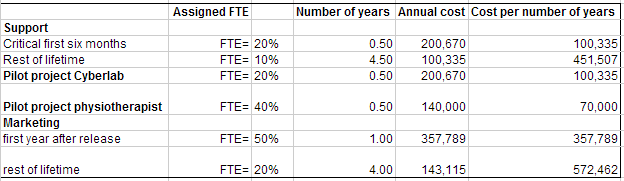
\includegraphics[scale=0.8]{calcFTE}
\label{fig:fte}
\end{center}
\end{figure}
\bigskip
\bigskip
\bigskip
\bigskip
\bigskip
\bigskip
\bigskip
\bigskip
\bigskip
\bigskip
\bigskip
\bigskip
\bigskip
\bigskip
\bigskip
\textbf{The cost of FTE=1 for the different employees} \\ \\

\begin{figure}
\begin{center}
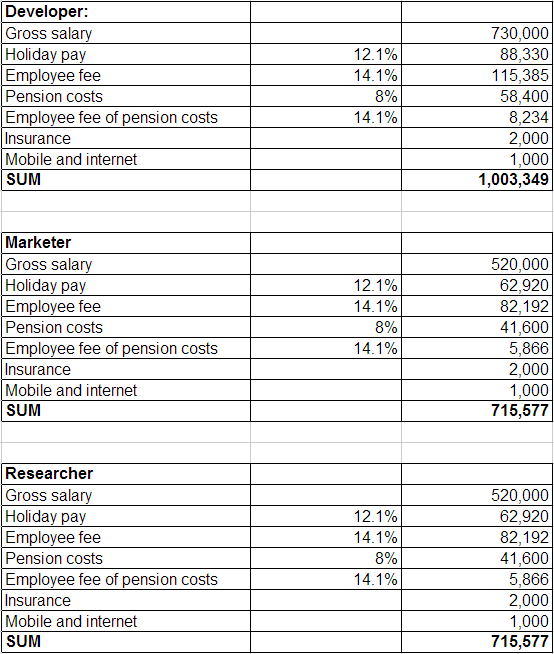
\includegraphics[scale=0.8]{appendixlonn}
\label{fig:employee}
\end{center}
\end{figure}


\newpage
\section*{Appendix F - Revenue Calculations}
\label{F}

The tables provided shows calculated revenue and profit. The 400 estimated units will be sold during a five year period, distributed by an s-curve. Present value (PV) has been calculated with a discount rate of 4 percent. We present income per year and total revenue for both the fixed price model and the usage fee model. We provide different price examples and solutions for both models. Total profit is calculated with an approximate total cost of 3 240 000 NOK, showed in Figure \ref{fig:profitRounded}. The same rounded total cost is used in all the calculations in the financial analysis. Figure \ref{fig:profitAll} shows the yearly and total profit for all examples with the actual cost of  3 238 775 NOK. \\ \\
\bigskip
\bigskip
\bigskip
\bigskip
\bigskip
\bigskip
\bigskip
\bigskip
\bigskip
\bigskip
\bigskip
\bigskip

\begin{figure}
\begin{center}
\includegraphics[scale=0.8]{revenuepvappendixfixed}
\caption{Revenue stream for three fixed price examples}
\label{fig:revenueFixed}
\end{center}
\end{figure}

\begin{figure}
\begin{center}
\includegraphics[scale=0.8]{revenuepvappendixusage}
\caption{Revenue stream for three usage fee examples}
\label{fig:revenueUsage}
\end{center}
\end{figure}

\begin{figure}
\begin{center}
\includegraphics[scale=0.8]{revenuepvappendixassumptations}
\caption{Discount rate of 4 percent and total cost of 3 240 000 NOK is used}
\label{fig:revenuePVassump}
\end{center}
\end{figure}

\begin{figure}
\begin{center}
\includegraphics[scale=0.8]{revenuepvappendixprofitrounded}
\caption{Total profit with the approximate total cost}
\label{fig:profitRounded}
\end{center}
\end{figure}

\begin{figure}
\begin{center}
\includegraphics[scale=0.8]{revenuepvappendixprofit}
\caption{Yearly and total profit for each example}
\label{fig:profitAll}
\end{center}
\end{figure}

\newpage
\section*{Appendix G - Beregning av potenstielt marked for Cyberlab}
\label{G}

We have calculated a potential marked for Cyberlab. We have done this by looking at four municipalities and the number of clinics (public and those with distribution from the government) in each of them. For each municipality we calculated number of inhabitants per clinic, and made an average of this. This average was compared to the total population in Norway. This gave us an estimate of 1 137 clinics in Norway. We rounded this up to 1 200 clinics.

\begin{figure}
\begin{center}
\includegraphics[scale=0.8]{antallklinikker}
\label{fig:clinics}
\end{center}
\end{figure}

\begin{figure}
\begin{center}
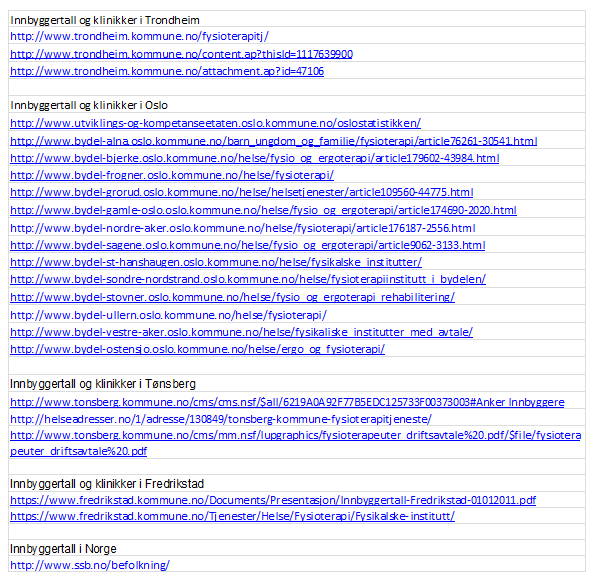
\includegraphics[scale=0.8]{kilder}
\label{fig:sources}
\end{center}
\end{figure}



